\documentclass[11pt,preprint, authoryear]{elsarticle}

\usepackage{lmodern}
%%%% My spacing
\usepackage{setspace}
\setstretch{1.2}
\DeclareMathSizes{12}{14}{10}{10}

% Wrap around which gives all figures included the [H] command, or places it "here". This can be tedious to code in Rmarkdown.
\usepackage{float}
\let\origfigure\figure
\let\endorigfigure\endfigure
\renewenvironment{figure}[1][2] {
    \expandafter\origfigure\expandafter[H]
} {
    \endorigfigure
}

\let\origtable\table
\let\endorigtable\endtable
\renewenvironment{table}[1][2] {
    \expandafter\origtable\expandafter[H]
} {
    \endorigtable
}


\usepackage{ifxetex,ifluatex}
\usepackage{fixltx2e} % provides \textsubscript
\ifnum 0\ifxetex 1\fi\ifluatex 1\fi=0 % if pdftex
  \usepackage[T1]{fontenc}
  \usepackage[utf8]{inputenc}
\else % if luatex or xelatex
  \ifxetex
    \usepackage{mathspec}
    \usepackage{xltxtra,xunicode}
  \else
    \usepackage{fontspec}
  \fi
  \defaultfontfeatures{Mapping=tex-text,Scale=MatchLowercase}
  \newcommand{\euro}{€}
\fi

\usepackage{amssymb, amsmath, amsthm, amsfonts}

\def\bibsection{\section*{References}} %%% Make "References" appear before bibliography


\usepackage[round]{natbib}

\usepackage{longtable}
\usepackage[margin=2.3cm,bottom=2cm,top=2.5cm, includefoot]{geometry}
\usepackage{fancyhdr}
\usepackage[bottom, hang, flushmargin]{footmisc}
\usepackage{graphicx}
\numberwithin{equation}{section}
\numberwithin{figure}{section}
\numberwithin{table}{section}
\setlength{\parindent}{0cm}
\setlength{\parskip}{1.3ex plus 0.5ex minus 0.3ex}
\usepackage{textcomp}
\renewcommand{\headrulewidth}{0.2pt}
\renewcommand{\footrulewidth}{0.3pt}

\usepackage{array}
\newcolumntype{x}[1]{>{\centering\arraybackslash\hspace{0pt}}p{#1}}

%%%%  Remove the "preprint submitted to" part. Don't worry about this either, it just looks better without it:
\makeatletter
\def\ps@pprintTitle{%
  \let\@oddhead\@empty
  \let\@evenhead\@empty
  \let\@oddfoot\@empty
  \let\@evenfoot\@oddfoot
}
\makeatother

 \def\tightlist{} % This allows for subbullets!

\usepackage{hyperref}
\hypersetup{breaklinks=true,
            bookmarks=true,
            colorlinks=true,
            citecolor=blue,
            urlcolor=blue,
            linkcolor=blue,
            pdfborder={0 0 0}}


% The following packages allow huxtable to work:
\usepackage{siunitx}
\usepackage{multirow}
\usepackage{hhline}
\usepackage{calc}
\usepackage{tabularx}
\usepackage{booktabs}
\usepackage{caption}


\newenvironment{columns}[1][]{}{}

\newenvironment{column}[1]{\begin{minipage}{#1}\ignorespaces}{%
\end{minipage}
\ifhmode\unskip\fi
\aftergroup\useignorespacesandallpars}

\def\useignorespacesandallpars#1\ignorespaces\fi{%
#1\fi\ignorespacesandallpars}

\makeatletter
\def\ignorespacesandallpars{%
  \@ifnextchar\par
    {\expandafter\ignorespacesandallpars\@gobble}%
    {}%
}
\makeatother

\newlength{\cslhangindent}
\setlength{\cslhangindent}{1.5em}
\newenvironment{CSLReferences}%
  {\setlength{\parindent}{0pt}%
  \everypar{\setlength{\hangindent}{\cslhangindent}}\ignorespaces}%
  {\par}


\urlstyle{same}  % don't use monospace font for urls
\setlength{\parindent}{0pt}
\setlength{\parskip}{6pt plus 2pt minus 1pt}
\setlength{\emergencystretch}{3em}  % prevent overfull lines
\setcounter{secnumdepth}{5}

%%% Use protect on footnotes to avoid problems with footnotes in titles
\let\rmarkdownfootnote\footnote%
\def\footnote{\protect\rmarkdownfootnote}
\IfFileExists{upquote.sty}{\usepackage{upquote}}{}

%%% Include extra packages specified by user

%%% Hard setting column skips for reports - this ensures greater consistency and control over the length settings in the document.
%% page layout
%% paragraphs
\setlength{\baselineskip}{12pt plus 0pt minus 0pt}
\setlength{\parskip}{12pt plus 0pt minus 0pt}
\setlength{\parindent}{0pt plus 0pt minus 0pt}
%% floats
\setlength{\floatsep}{12pt plus 0 pt minus 0pt}
\setlength{\textfloatsep}{20pt plus 0pt minus 0pt}
\setlength{\intextsep}{14pt plus 0pt minus 0pt}
\setlength{\dbltextfloatsep}{20pt plus 0pt minus 0pt}
\setlength{\dblfloatsep}{14pt plus 0pt minus 0pt}
%% maths
\setlength{\abovedisplayskip}{12pt plus 0pt minus 0pt}
\setlength{\belowdisplayskip}{12pt plus 0pt minus 0pt}
%% lists
\setlength{\topsep}{10pt plus 0pt minus 0pt}
\setlength{\partopsep}{3pt plus 0pt minus 0pt}
\setlength{\itemsep}{5pt plus 0pt minus 0pt}
\setlength{\labelsep}{8mm plus 0mm minus 0mm}
\setlength{\parsep}{\the\parskip}
\setlength{\listparindent}{\the\parindent}
%% verbatim
\setlength{\fboxsep}{5pt plus 0pt minus 0pt}



\begin{document}



\begin{frontmatter}  %

\title{Helping You Write Academic Papers in R using Texevier}

% Set to FALSE if wanting to remove title (for submission)




\author[Add1]{Nico Katzke\footnote{\textbf{Contributions:}
  \newline \emph{The authors would like to thank no institution for
  money donated to this project. Thank you sincerely.}}}
\ead{nfkatzke@gmail.com}

\author[Add1,Add2]{John Smith}
\ead{John@gmail.com}

\author[Add1,Add2]{John Doe}
\ead{Joe@gmail.com}



\address[Add1]{Prescient Securities, Cape Town, South Africa}
\address[Add2]{Some other Institution, Cape Town, South Africa}

\cortext[cor]{Corresponding author: Nico Katzke\footnote{\textbf{Contributions:}
  \newline \emph{The authors would like to thank no institution for
  money donated to this project. Thank you sincerely.}}}

\begin{abstract}
\small{
Abstract to be written here. The abstract should not be too long and
should provide the reader with a good understanding what you are writing
about. Academic papers are not like novels where you keep the reader in
suspense. To be effective in getting others to read your paper, be as
open and concise about your findings here as possible. Ideally, upon
reading your abstract, the reader should feel he / she must read your
paper in entirety.
}
\end{abstract}

\vspace{1cm}


\begin{keyword}
\footnotesize{
Multivariate GARCH \sep Kalman Filter \sep Copula \\
\vspace{0.3cm}
}
\footnotesize{
\textit{JEL classification} L250 \sep L100
}
\end{keyword}



\vspace{0.5cm}

\end{frontmatter}



%________________________
% Header and Footers
%%%%%%%%%%%%%%%%%%%%%%%%%%%%%%%%%
\pagestyle{fancy}
\chead{}
\rhead{}
\lfoot{}
\rfoot{\footnotesize Page \thepage}
\lhead{}
%\rfoot{\footnotesize Page \thepage } % "e.g. Page 2"
\cfoot{}

%\setlength\headheight{30pt}
%%%%%%%%%%%%%%%%%%%%%%%%%%%%%%%%%
%________________________

\headsep 35pt % So that header does not go over title




\begin{verbatim}
## Q(m) of squared series(LM test):  
## Test statistic:  6266.108  p-value:  0 
## Rank-based Test:  
## Test statistic:  1487.596  p-value:  0 
## Q_k(m) of squared series:  
## Test statistic:  13012.78  p-value:  0 
## Robust Test(5%) :  1770.574  p-value:  0
\end{verbatim}

The MARCH test indicates that all the MV portmanteau tests reject the
null of no conditional heteroskedasticity, motivating our use of MVGARCH
models. Let's set up the model

\begin{verbatim}
## Test results:  
## Q(m) of et: 
## Test and p-value:  67.86301 1.144478e-10 
## Rank-based test: 
## Test and p-value:  45.01247 2.163493e-06 
## Qk(m) of epsilon_t: 
## Test and p-value:  251.1729 5.494596e-06 
## Robust Qk(m):  
## Test and p-value:  149.6698 0.7098375
\end{verbatim}

\begin{verbatim}
## , , 2010-01-01
## 
##           MSCI_ACWI   US_10Yr   MSCI_RE Oil_Brent
## MSCI_ACWI 1.0000000 0.3672945 0.6989608 0.3916873
## US_10Yr   0.3672945 1.0000000 0.1060070 0.2437526
## MSCI_RE   0.6989608 0.1060070 1.0000000 0.2554721
## Oil_Brent 0.3916873 0.2437526 0.2554721 1.0000000
## 
## , , 2010-01-04
## 
##           MSCI_ACWI   US_10Yr   MSCI_RE Oil_Brent
## MSCI_ACWI 1.0000000 0.3669617 0.6988083 0.3913564
## US_10Yr   0.3669617 1.0000000 0.1055386 0.2433507
## MSCI_RE   0.6988083 0.1055386 1.0000000 0.2550748
## Oil_Brent 0.3913564 0.2433507 0.2550748 1.0000000
## 
## , , 2010-01-05
## 
##           MSCI_ACWI   US_10Yr   MSCI_RE Oil_Brent
## MSCI_ACWI 1.0000000 0.3340547 0.6777565 0.4364434
## US_10Yr   0.3340547 1.0000000 0.1027695 0.2291449
## MSCI_RE   0.6777565 0.1027695 1.0000000 0.2623880
## Oil_Brent 0.4364434 0.2291449 0.2623880 1.0000000
\end{verbatim}

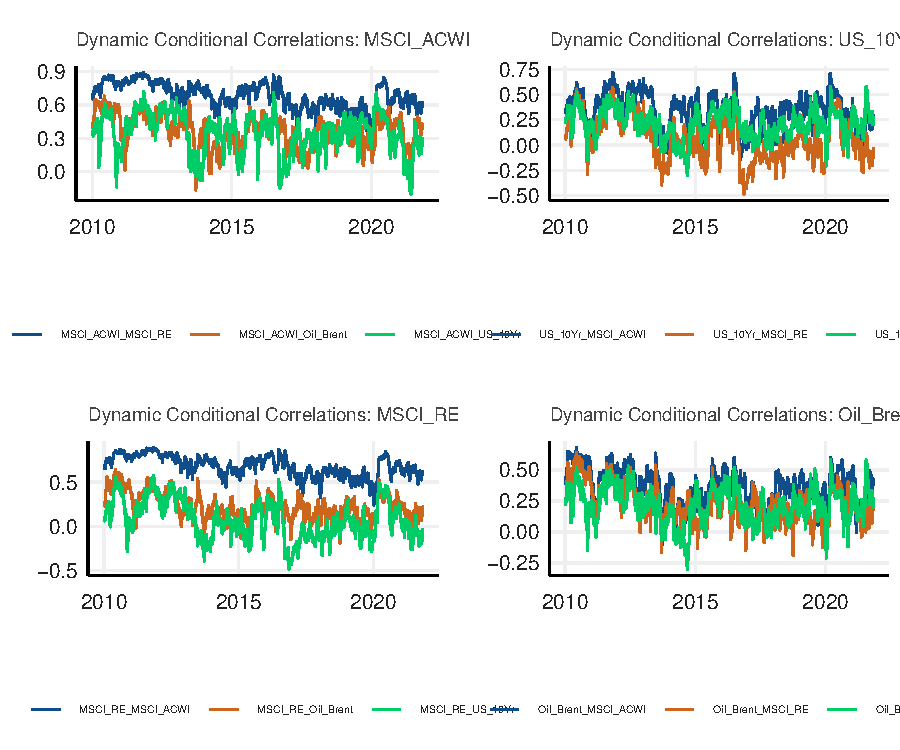
\includegraphics{Question6_files/figure-latex/unnamed-chunk-7-1.pdf}

\hypertarget{go-garch}{%
\section{Go Garch}\label{go-garch}}

\begin{verbatim}
## 
## *------------------------------*
## *        GO-GARCH Fit          *
## *------------------------------*
## 
## Mean Model       : CONSTANT
## GARCH Model      : sGARCH
## Distribution : mvnorm
## ICA Method       : fastica
## No. Factors      : 4
## No. Periods      : 3086
## Log-Likelihood   : 38671.96
## ------------------------------------
## 
## U (rotation matrix) : 
## 
##        [,1]   [,2]    [,3]    [,4]
## [1,]  0.859 -0.359 -0.2106 -0.2992
## [2,]  0.398  0.277 -0.0869  0.8704
## [3,] -0.187 -0.882  0.1952  0.3854
## [4,]  0.264  0.127  0.9539 -0.0656
## 
## A (mixing matrix) : 
## 
##          [,1]    [,2]      [,3]      [,4]
## [1,] -0.00140 0.00865  0.002277  0.000678
## [2,] -0.02864 0.00726  0.006998  0.002690
## [3,] -0.00139 0.00877 -0.003286 -0.000216
## [4,] -0.00201 0.00728  0.000874  0.020820
\end{verbatim}

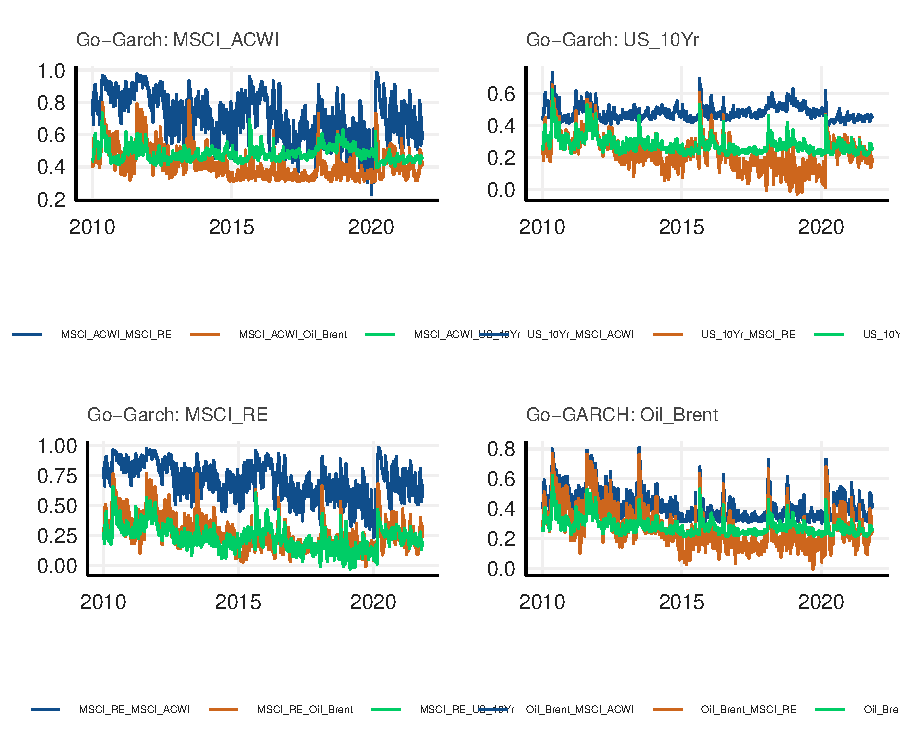
\includegraphics{Question6_files/figure-latex/unnamed-chunk-10-1.pdf}

\begin{verbatim}
##                  PC1        PC2         PC3         PC4
## MSCI_ACWI -0.6080549  0.2681471  0.01713371 -0.74704269
## MSCI_RE   -0.5540251  0.5226063  0.09680532  0.64075547
## Oil_Brent -0.3932987 -0.6563281  0.63617819  0.09913059
## US_10Yr   -0.4106600 -0.4735115 -0.76525321  0.14674050
\end{verbatim}

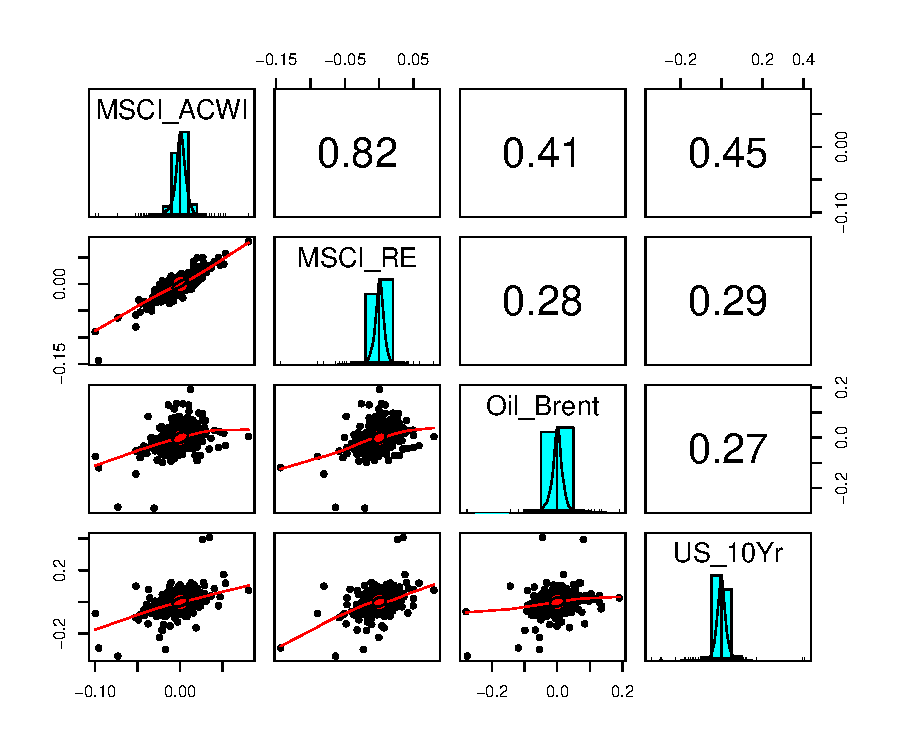
\includegraphics{Question6_files/figure-latex/unnamed-chunk-11-1.pdf}

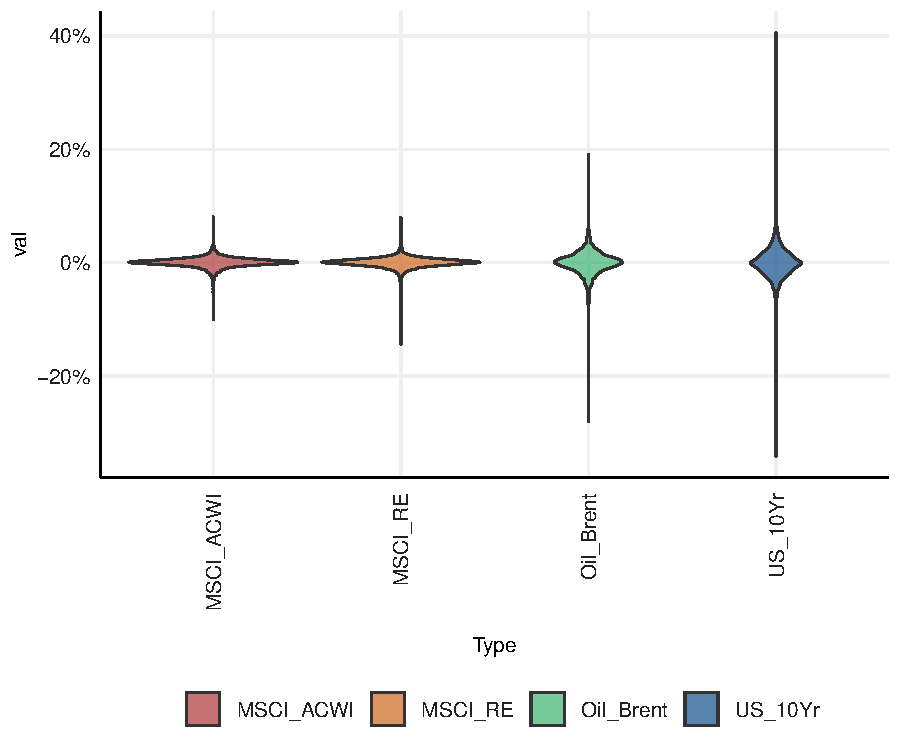
\includegraphics{Question6_files/figure-latex/unnamed-chunk-12-1.pdf}

The US 10 year bond shows the highest degree of dispersion, followed by
Oil, and clearly follows a different distribution process to the other
two indices.

\newpage

\hypertarget{references}{%
\section*{References}\label{references}}
\addcontentsline{toc}{section}{References}

\hypertarget{refs}{}
\begin{CSLReferences}{0}{0}
\end{CSLReferences}

\hypertarget{appendix}{%
\section*{Appendix}\label{appendix}}
\addcontentsline{toc}{section}{Appendix}

\hypertarget{appendix-a}{%
\subsection*{Appendix A}\label{appendix-a}}
\addcontentsline{toc}{subsection}{Appendix A}

Some appendix information here

\hypertarget{appendix-b}{%
\subsection*{Appendix B}\label{appendix-b}}
\addcontentsline{toc}{subsection}{Appendix B}

\bibliography{Tex/ref}





\end{document}
